\section{Číselné soustavy, převody}
\label{sec:ciselnesoustavy}
Čísla se skládají z číslic.
Číslo 49 z číslic 4 a 9.
Reálnou hodnotu takového čísla neznáme jelikož víme že každá pozice označuje násobek základního čísla soustavy umocněné podle řádu, ale nevíme které soustavy.
V naší (desítkové) soustavě by se jednal o součet: $4*10^1 + 9*10^0$, mezitím co v jiné například: $4*16^1 + 9*16^0$.
Jestliže bychom k tomuto číslu v naší soustavě přidali 1, tak by vzniklo číslo 50, jelikož v naší soustavě nemáme čísliči větší jak 9.
Existují však soustavy, kde existují číslice větší než 9 - například F, takové soustavě se říká hexademialní a používáme ji v informatice a dokonce i soustavy kde nejvyšší číslice je 1 - takové soustavě říkáme binární a také ji používáme v informatice.
\subsection{Převody mezi soustavami}
\subsubsection{Převod z desítkové soustavy}
Z desítkové číselné soustavy převádíme do jakékoli jiné soustavy tak, že desítkové číslo dělíme základem dané číselné soustavy a sepisujeme zbytky po dělení.
Poslední získaná číslice je nejvyšší řád čísla nové soustavy.
\subsubsection{Převod desetinných míst}
Destinné číslo si rozdělíme na dvě čísla oddělené destinnou čárkou a ty samostatně převedeme a vrátíme mezi ně desetinnou čárku.
Desetinnou část ovšem místo dělení násobíme a výsledky poustupně sčítáme.
Poslední získaná číslice je nejnižší řád čísla nové soustavy.
Desetinnou část násobíme dokud nedostaneme buďto nulový výsledek, určtený počet destinných míst nebo napříkal tři nuly po sobě.
\subsubsection{Převod z binární soustavy}
Pro převod z binární soutavy do osmičkové nebo šestnáctkové soustavy rozdělujeme samotné binární číslo do trojic pro osmičkovou nebo čtveřic pro šestnáctkovou a tyto skupiny následně převádíme a řadíme za sebe podle řádu.
Pro převod do desítkové soustavy sečítáme jednotlivé hodnoty číslic.
\subsubsection{Před do binární soustavy}
Pro převod z osmičkové nebo šestnáctkové soustavy do binární musíme každou číslici převést do binární soustavy a seřadit čísla za sebou.
\subsection{Ukládání desetinných čísel}
Pro zobrazení reálných, velmi malých a nebo velmi velkých číšel se používá pohyblivá řádka.
Formát takového čísla bývá: $x = M*z^E$.
M = mantissa, E = exponent (v obrázku "fraction"), z = základ (2), x = výsledek.
K jeho zápisu nám slouží \textbf{Single precision formát}, která ukladá tyto hodnoty ve 4 bajtech paměti.\\

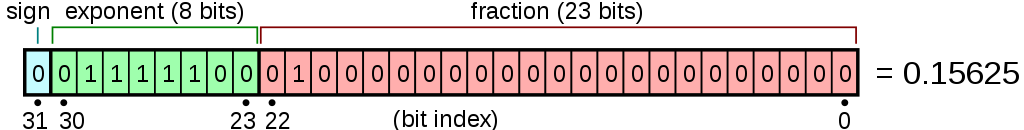
\includegraphics[width=\linewidth]{TVY-POS/Ciselne-soustavy/single_precision.png}\\

Základ čísla se neukládá, ale místo něho můžeme na posledním bitu vidět znaménkový bit pro určení záportného čísla.
Exponent se ukladá ve tvaru od -126 do 127, kde hodnota 128 představuje nulu.
Hodnoty -127 (Samé 0) a 128 (Samé 1) jsou používány pro speciální čísla (nenašel jsem).
Existují také další precision formáty, které ukládají čísla na větší místo v paměti (64bit, 128bit) určené pro přesnější čísla.
